\chapter{Testing programs}

A software bug is an error in a computer program that causes it to produce an incorrect result or behave in an unintended manner. The term bug was used by Thomas Edison in 1878\footnote{\url{https://en.wikipedia.org/wiki/Software_bug}, possibly \url{http://edison.rutgers.edu/NamesSearch/DocImage.php3?DocId=LB003487}}, but made popular in computer science by Grace Hopper, who found a moth interferring with the electronic circuits of the Harward Mark II electromechanical computer and coined the term \idx{bug} for errors in computer programs. The original bug is shown in Figure~\ref{fig:bug}.
\begin{figure}
  \centering
  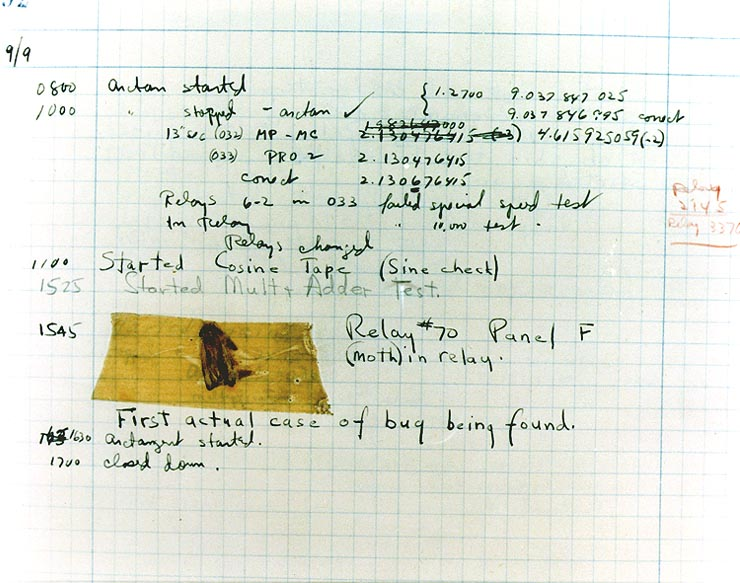
\includegraphics[width=0.45\linewidth]{H96566k}
  \caption{The first computer bug caught by Grace Hopper, U.S. Naval Historical Center Online Library Photograph NH 96566-KN.}
  \label{fig:bug}
\end{figure}
Software is everywhere, and errors therein have huge economic impact on our society and can threaten lives\footnote{\url{https://en.wikipedia.org/wiki/List_of_software_bugs}}.

The ISO/IEC organizations have developed standards for software testing\footnote{ISO/IEC 9126, International standard for the evaluation of software quality, December 19, 1991, later replaced by ISO/IEC 25010:2011}.  To illustrate basic concepts of software quality consider a hypothetical route planning system. Essential factors of its quality is,
\begin{description}
\item[Functionality:]\idxs{functionality} Does the software compile and run without internal errors. Does it solve the problem, it was intended to solve? E.g., does the route planning software finde a suitable route from point a to b?
\item[Reliability:]\idxs{reliability} Does the software work reliably over time? E.g., does the route planning software work in case of internet dropouts?
\item[Usability:]\idxs{usability} Is the software easy and intuitive to use by humans? E.g., is it easy to enter adresses and alternative routes in the software's interface?
\item[Efficiency:]\idxs{efficiency} How many computer and human resources does the software require? E.g., does it take milliseconds or hours to find a requested route? Can the software run on a mobile platform with limited computer speed and memory?
\item[Maintainability:]\idxs{maintainability} In case of the discovery of new bugs, is it easy to test and correct the software? Is it easy to extend the software with new functionality? E.g., is it easy to update the map with updated roadmaps and new information? Can the system be improved to work both for car drivers and bicyclists? 
\item[Portability:]\idxs{portability} Is it easy to port the software to new systems such as new server architecture and screen sizes? E.g., if the routing software originally was written for IOS devices, will it be easy to port to Android systems?
\end{description}
The above mentioned concepts are ordered based on the requirements of the system. Functionality and reliability ares perhaps the most important concepts, since if the software does not solve the specified problem, then the software designing process has failed. However, many times the problem definition will evolve along with the software development process. But as a bare minimum, the software should run without internal errors and not crash under well defined set of circumstances. Further, it is often the case, that software designed for the general public requires a lot of attention to the usability of the software, since in many cases non-experts are expected to be able to use the software little or no prior training. On the other hand, software used internally in companies will be used by a small number of people, who become experts in using the software, and it is often less important that the software is easy to understand by non-experts. An example is text processing software Microsoft Word versus Gnu Emacs and LaTeX. Word is designed to be used by non-experts for small documents such as letters and notes, and relies heavily on interfacing with the system using click-interaction. On the other hand, Emacs and LaTeX are for experts for longer and professionally typeset documents, and relies heavily on keyboard shortcuts and text-codes for typesetting document entities. 

The purpose of \idx{software testing} is to find bugs. For errors found we engage in \idx{debugging}, which is the process of diagnosing and correcting bugs. Once we have a failed software test, i.e., one that does not find any bugs, then we have strengthened our belief in the software, but it is important to note, that software testing and debugging rarely removes all bugs, and with each correction or change of software, there is a fair chance of introducing new bugs. It is not exceptional, that the software testing the software is as large as the original.

In this chapter, we will focus on two approaches to software testing, which emphasizes functionality: \idx[white-box testing]{white-box} and \idx{black-box testing}. An important concept in this context is \idx{unit testing}, where the program is considered in smaller pieces, called units, and for which accompanying programs for testing can be made, which tests these units automatically. Black-box testing considers the problem formulation and the program interface, and can typically be written early in the software design phase. In contrast, white-box testing considers the program text, and thus requires the program to be available. Thus there is a tendency for black-box test programs to be more stable, while white-box testing typically is developed incrementally along side the software development.

To illustrate software testing we'll start with a problem:
\begin{problem}
  Given any date in the Gregorian calendar, calculate the day of week.
\end{problem}
Facts about dates in the Gregorian calendar are:
\begin{itemize}
\item combinations of dates and weekdays repeat themselves every 400 years;
\item the typical length of the months Januar, February, \dots follow the knucle rule, i.e., January belongs to the index knuckle, February to the space between the index and the middle finger, and August restarts or starts on the other hand. All knuckle months have 31 days, all spacing months have 30 days except February, which has 29 days on leap years and 28 days all other years.
\item A leap year is a multiplum of 4, except if it is also a multiplum of 100 but not of 400.
\end{itemize}
Many solutions to the problem have been discovered, and here we will base our program on Gauss' method, which is based on integer division and calculates the weekday of the 1st of January of a given year. For any other date, we will count our way through the weeks from the previous 1st of January. The algorithm relies on an enumeration of weekdays starting with Sunday = 0, Monday = 1, \dots, and Saturday = 6. Our proposed solution is,
  %
  \fse{date2Day}{A function that can calculate day-of-week from any date in the Gregorian calendar.}
  %
  %To solve this problem, we are going to implement the Doomsday algorithm by John Conway\footnote{\url{http://www.timeanddate.com/date/doomsday-weekday.html}}. The algorithm is based on the fact that calendars repeat themselves every 400 years, and within a cycle, certain dates are always the same day of week. For the 400 year cycle, 1800-2199, the algorithm uses anchor days: 1800 - 1899: Friday, 1900 - 1999: Wednesday, 2000 - 2099: Tuesday, and 2100 - 2199: Sunday. For a given date (dd, mm, yyyy), the algorithm calculates the Doomsday of the year in question as by 6 steps:
% \begin{enumerate}
% \item Let $a$ be the integer division of the last two digits of yyyy by 12
% \item Let $b$ be the remainder of the last two digits of yyyy by 12
% \item Let $c$ be the integer division of $b$ by 4
% \item Let $d$ be the anchor number of yyyy
% \item Let $e$ be the remainder of $a+b+c+d$ by 7. This is the doomsday.
% \item count weekdays from nearest doomsday.
% \end{enumerate}

\section{White-box testing}
\idx[white-box testing]{White-box testing} considers the text of a program. The degree to which the text of the program is covered in the test is called \idx{coverage}. Since our program is small, we do have the opportunity to ensure that all functions are called at least once, which is called \idx{function coverage}, we will also be able to test every branching in the program, which is called \idx{branching coverage}, an in this case that implies \idx{statement coverage}. The procedure is as follows:
\begin{enumerate}
\item Decide which are the units to test: The program shown in Listing~\ref{date2Day} has 3 functions, and we will consider these each as a unit, but we might as well just have chosen \lstinline!date2Day! as a single unit. The important part is that the union of units must cover the whole program text, and since \lstinline!date2Day! calls both \lstinline!januaryFirstDay! and \lstinline!sum!, designing test cases for the two later is superfluous. However, we may have to do this anyway, when debugging, and we may choose at a later point to use these functions separately, and in both cases we will be able to reuse the testing of the smaller units.
\item Identify branching points: The function \lstinline!januaryFirstDay! has no branching function, \lstinline!sum! has one, and depending on the input values two paths through the code may be used, and \lstinline!date2Day! has one, where the number of days in February is decided. Note that in order to test this, our test-date must be March 1 or later. In this example, there are only examples of \keyword{if}-branch points, but they may as well be loops and pattern matching expressions. In the following code, the branch points have been given a comment and a number,
  % 
  \fse{date2DayAnnotated}{In white-box testing, the branch points are identified.}
  % 
 \item For each unit, produce an input set that tests each branches: In our example the branch points depends on a boolean expression, and for good measure, we are going to test each term that can lead to branching. Thus,
   \begin{center}
     \begin{tabularx}{\linewidth}{|l|l|l|l|X|}
     \hline
     Unit & Branch & Condition & Input & Expected output\\
     \hline
       \lstinline{januaryFirstDay} & 0 & -& \lstinline{2016} & \lstinline{5}\\
     \hline
     \lstinline{sum} 
       & 1 & \lstinline{0 <= j \&\& j < lst.Length} &&\\
       & 1a & \lstinline{true \&\& true} & \lstinline{[1; 2; 3] 1} & \lstinline{3}\\
       & 1b & \lstinline{false \&\& true} & \lstinline{[1; 2; 3] -1} & \lstinline{0}\\
       & 1c & \lstinline{true \&\& false} & \lstinline{[1; 2; 3] 10} & \lstinline{0}\\
       & 1d & \lstinline{false \&\& false} & - & -\\
       \hline
       \lstinline{date2Day} & 1 & \lstinline{(y \% 4 = 0)}  &  & \\
          & & \hspace*{5mm}\lstinline{\&\& ((y \% 100 <> 0)} &  & \\
          & & \hspace*{10mm}\lstinline{|| (y \% 400 = 0))} &  & \\
        & - & \lstinline{true \&\& (true || true)} & - & -\\
        & 1a & \lstinline{true \&\& (true || false)} & \lstinline{8 9 2016} & \lstinline{Thursday}\\
        & 1b & \lstinline{true \&\& (false || true)} & \lstinline{8 9 2000} & \lstinline{Friday}\\
        & 1c & \lstinline{true \&\& (false || false)} & \lstinline{8 9 2100} & \lstinline{Wednesday}\\
        & - & \lstinline{false \&\& (true || true)} & - & -\\
        & 1d & \lstinline{false \&\& (true || false)} & \lstinline{8 9 2015} & \lstinline{Tuesday}\\
        & - & \lstinline{false \&\& (false || true)} & - & -\\
        & - & \lstinline{false \&\& (false || false)} & - & -\\
       \hline
     \end{tabularx}
   \end{center}
   The impossible cases have been intentionally blank, e.g., it is not possible for $j<0$ and $j>n$ for some positive value $n$.
 \item Write a program, that test all these cases and checks the output, e.g.,
   % 
   \fsa{date2DayWhiteTest}{firstline=22}{The tests identified by white-box analysis. The program from Listing~\ref{date2DayAnnotated} has been omitted for brevity.}
   % 
\end{enumerate}
Notice, that the output of the tests are organized such that they are enumerated per unit, hence we can rearrange as we like and still uniquely refer to a unit's test. Also, the output of the test program produces a list of tests, that should return true or success or a similar positively loaded word, but without further or only little detail, such that we at a glance can identify any test that produced unexpected results.

After the white-box testing has failed to find errors in the program, we have some confidence in the program, since we have run every line at least once. It is, however, in no way a guarantee, that the program is error free, which is why white-box testing is often accompanied with black-box testing to be described next.

\section{Back-box testing}
In black-box testing the program is considered a black box, and no knowledge is required about how a particular problem is solved, in fact, it is often useful not to have that knowledge at all. It is rarely possible to test all input to a program, so in black-box testing, the solution is tested for typical and extreme cases based on knowledge of the problem. The procedure is as follows:
\begin{enumerate}[label=]
\item Decide on the interface to use: It is useful to have an agreement with the software developers about what interface is to be used, e.g., in our case, the software developer has made a function \lstinline!date2Day d m y!, where \lstinline!d!, \lstinline!m!, and \lstinline!y! are integers specifying the day, month, and year.
\item Make an overall description of the tests to be performed and their purpose:
  \begin{enumerate}[label=\arabic*]
  \item\label{allWeekDays} a consecutive week, to ensure that all weekdays are properly returned
  \item\label{crossBondaries} two set of consecutive days across boundaries that may cause problems: across a new year, across a regular month boundary.
  \item\label{februaryBoundaries} a set of consecutive days across February-March boundaries for a leap and non-leap year
  \item\label{leapYears} four dates after february in a non-multiplum-of-100 leap year and in a non-leap year, a multiplum-of-100-but-not-of-400 leap year, and a multiplum-of-100-but-and-of-400 leap year.
  \end{enumerate}
  Given no information about the program's text, there are other dates, that one could consider as likely candidates of errors, but the above is judged to be a fair coverage.
\item Choose a specific set of input and expected output relations on tabular form:
\begin{center}
  \begin{tabular}{|l|r|l|}
    \hline
    Test number&Input& Expected output\\
    \hline
    \ref{allWeekDays}a&1 1 2016&Friday\\
    \ref{allWeekDays}b&2 1 2016&Saturday\\
    \ref{allWeekDays}c&3 1 2016&Sunday\\
    \ref{allWeekDays}d&4 1 2016&Monday\\
    \ref{allWeekDays}e&5 1 2016&Tuesday\\
    \ref{allWeekDays}f&6 1 2016&Wednesday\\
    \ref{allWeekDays}g&7 1 2016&Thursday\\
    \hline
    \ref{crossBondaries}a&31 12 2014&Wednesday\\
    \ref{crossBondaries}b&1 1 2015&Thursday\\
    \ref{crossBondaries}c&30 9 2017&Saturday\\
    \ref{crossBondaries}d&1 10 2017&Sunday\\
    \hline
    \ref{februaryBoundaries}a&28 2 2016&Sunday\\
    \ref{februaryBoundaries}b&29 2 2016&Monday\\
    \ref{februaryBoundaries}c&1 3 2016&Tuesday\\
    \ref{februaryBoundaries}d&28 2 2017&Tuesday\\
    \ref{februaryBoundaries}e&1 3 2017&Wednesday\\
    \hline
    \ref{leapYears}a&1 3 2015&Sunday\\
    \ref{leapYears}b&1 3 2012&Thursday\\
    \ref{leapYears}c&1 3 2000&Wednesday\\
    \ref{leapYears}d&1 3 2100&Monday\\
    \hline
  \end{tabular}
\end{center}
\item Write a program executing the tests:
  % 
  \fsa{date2DayBlackTest}{firstline=22}{The tests identified by black-box analysis. The program from Listing~\ref{date2DayAnnotated} has been omitted for brevity.}
  % 
  Notice how the program has been made such that it is almost a direct copy of the table, produced in the previous step.
\end{enumerate}
A black-box test is a statement of what a solution should fulfill for a given problem. Hence, \advice{it is a good idea to make a black-box test early in the software design phase, in order to clarify the requirements for the code to be developed, and take an outside view of the code prior to developing it.}

After the black-box testing has failed to find errors in the program, we have some confidence in the program, since from a user's perspective, the program produces sensible output in many casses. It is, however, in no way a guarantee, that the program is error free.

\begin{comment}
  http://www.scientificamerican.com/article/pogue-5-most-embarrassing-software-bugs-in-history/, 5 Most Embarrassing Software Bugs in History

  http://royal.pingdom.com/2009/03/19/10-historical-software-bugs-with-extreme-consequences/

  https://raygun.com/blog/2014/05/10-costly-software-errors-history/

  http://www.computerworld.com/article/2515483/enterprise-applications/epic-failures--11-infamous-software-bugs.html

  http://catless.ncl.ac.uk/Risks/20.59.html#subj1

  https://en.wikipedia.org/wiki/List_of_software_bugs

  December 19, 1991; ISO/IEC 9126, international standard for the evaluation of software quality, replaced by ISO/IEC 25010:2011. Not publicly available, \footnote{A review of the ISO/IEC 9126 is given in \url{http://www.sqa.net/iso9126.html}. A brief review of ISO/IEC 25010:2011 is given in }
\end{comment}

\jon{Possibly add examples of debugging.}

%%% Local Variables:
%%% TeX-master: "fsharpNotes"
%%% End:
